\section{Formgedächtnislegierungen}

\begin{frame}[t]\frametitle{Gliederung: Formgedächtnislegierungen}
\tableofcontents[
currentsection,
subsectionstyle=show/show/hide
]
\end{frame}

\begin{frame}[c]\frametitle{NITINOL}
	\centering
	Nickel Titanium Naval Ordnance Laboratory.
	\\
	Durch zufall 1958 entdeckt.
\end{frame}


 \label{ergb:01}
 \begin{frame}[c]\frametitle{Beispiel Büroklammer}
	\centering
	\begin{figure}
		\begin{minipage}{0.45\textwidth}
		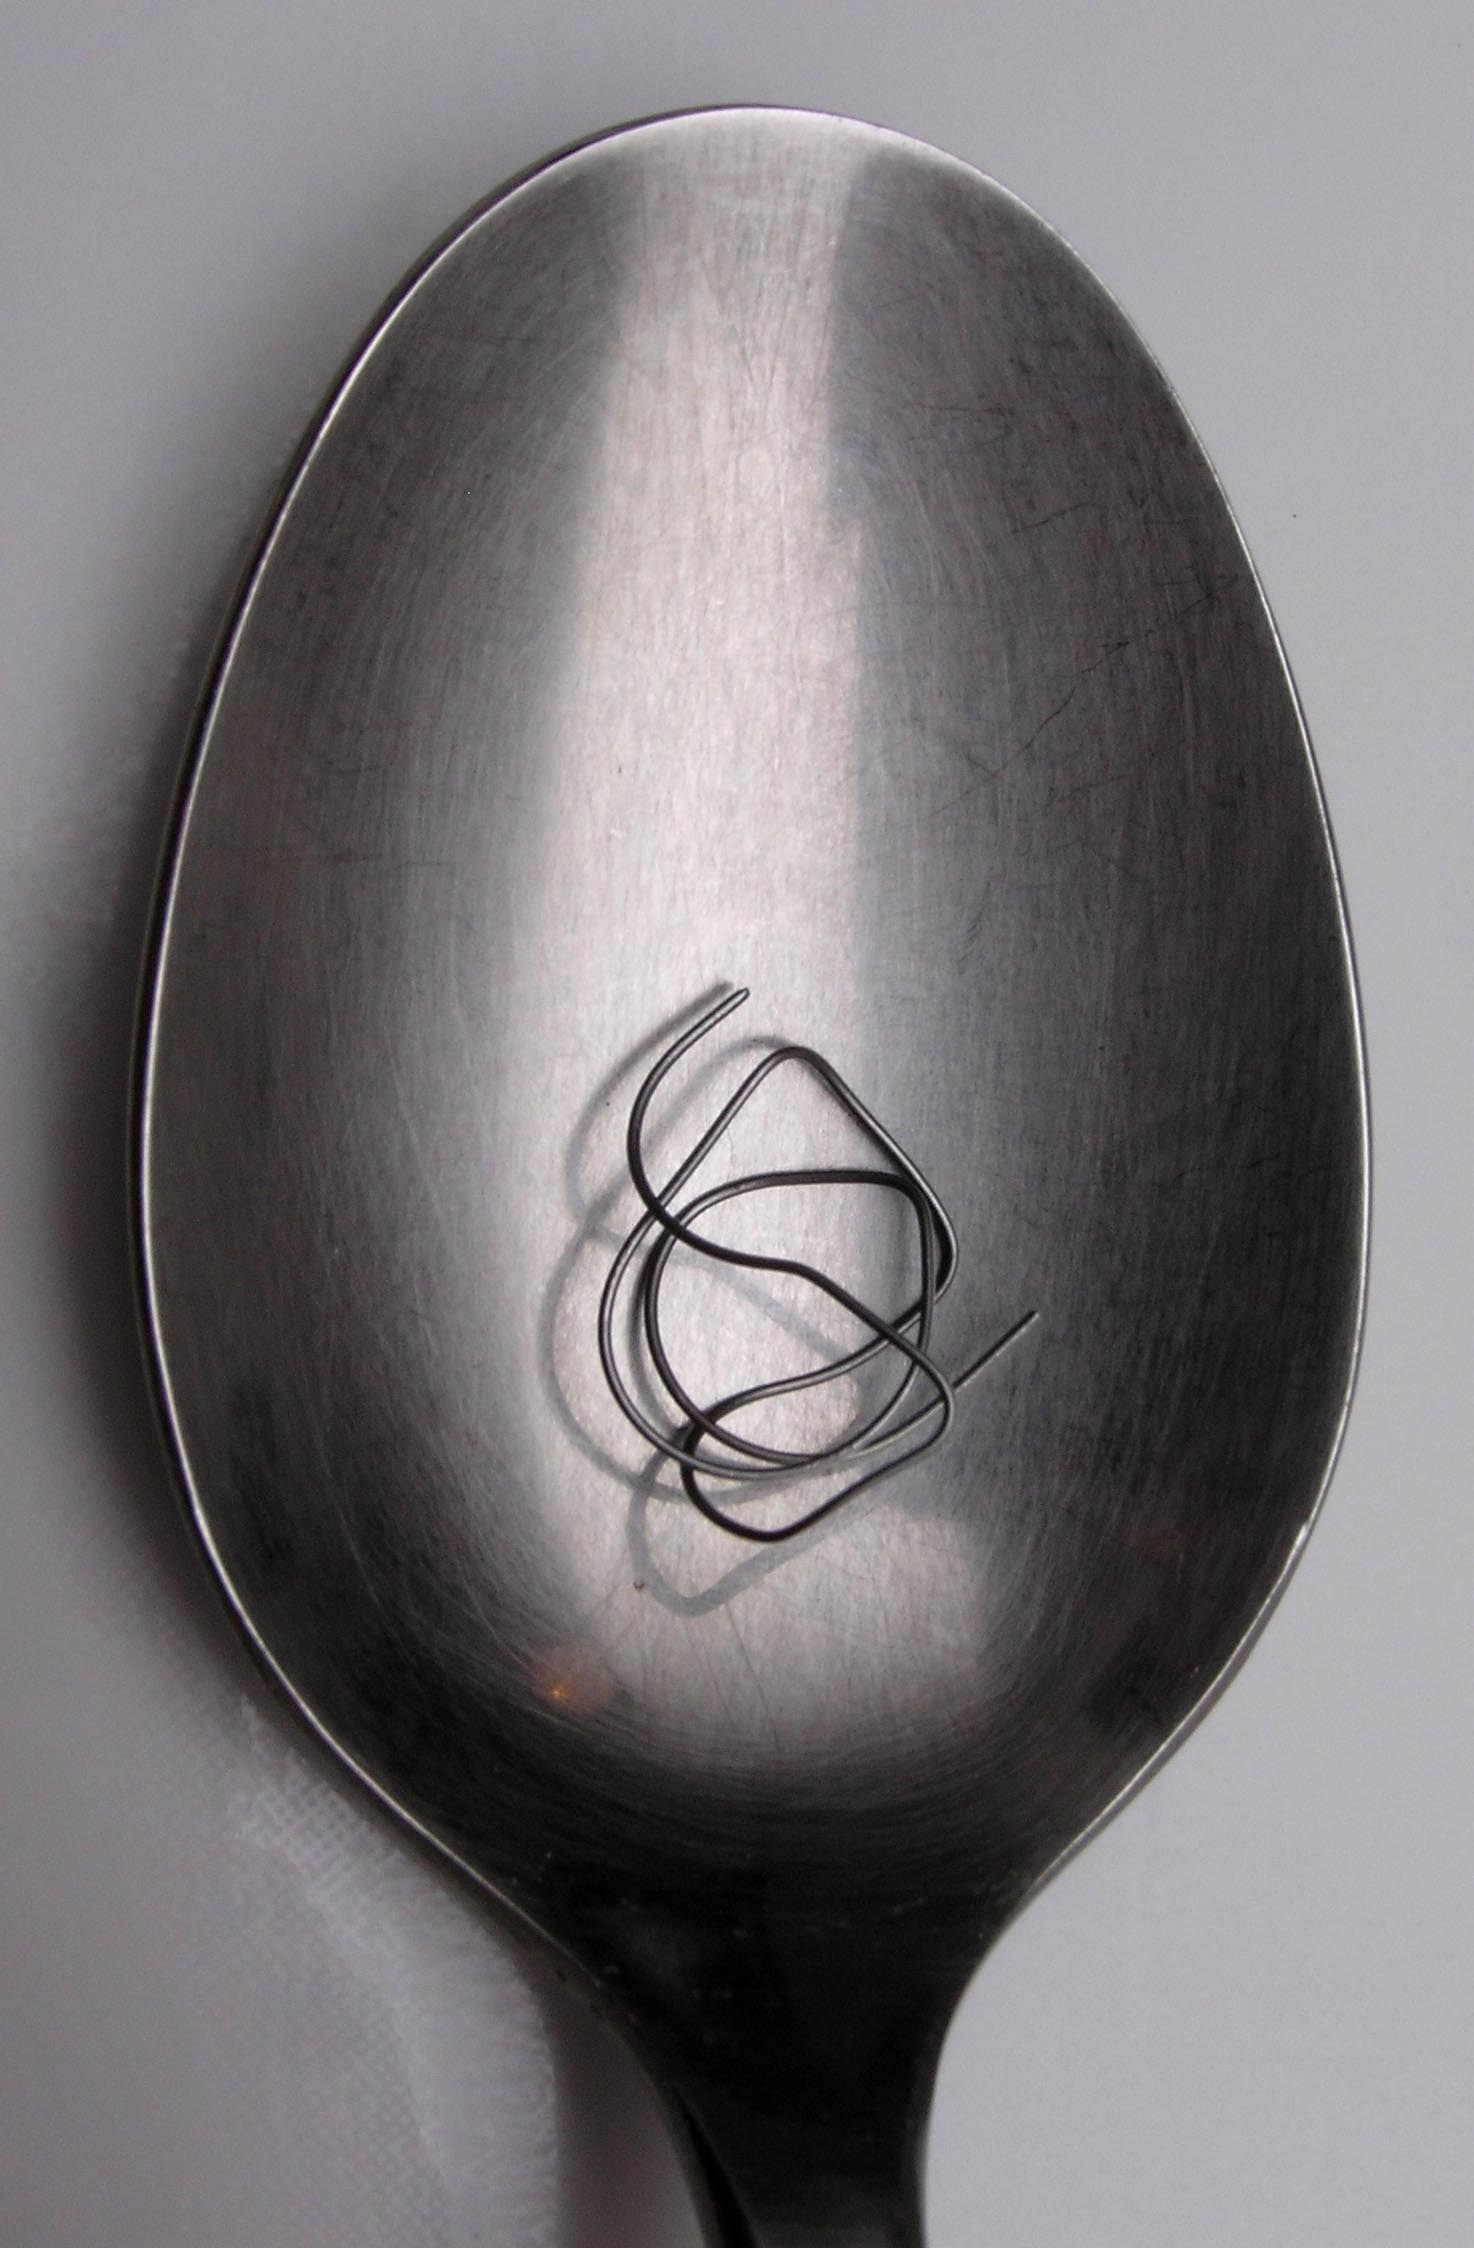
\includegraphics[width=0.5\textwidth]{medien/Nitinol_bueroklammer_verbogen.jpg}
		\end{minipage}
	\hfill
		\begin{minipage}{0.45\textwidth}
		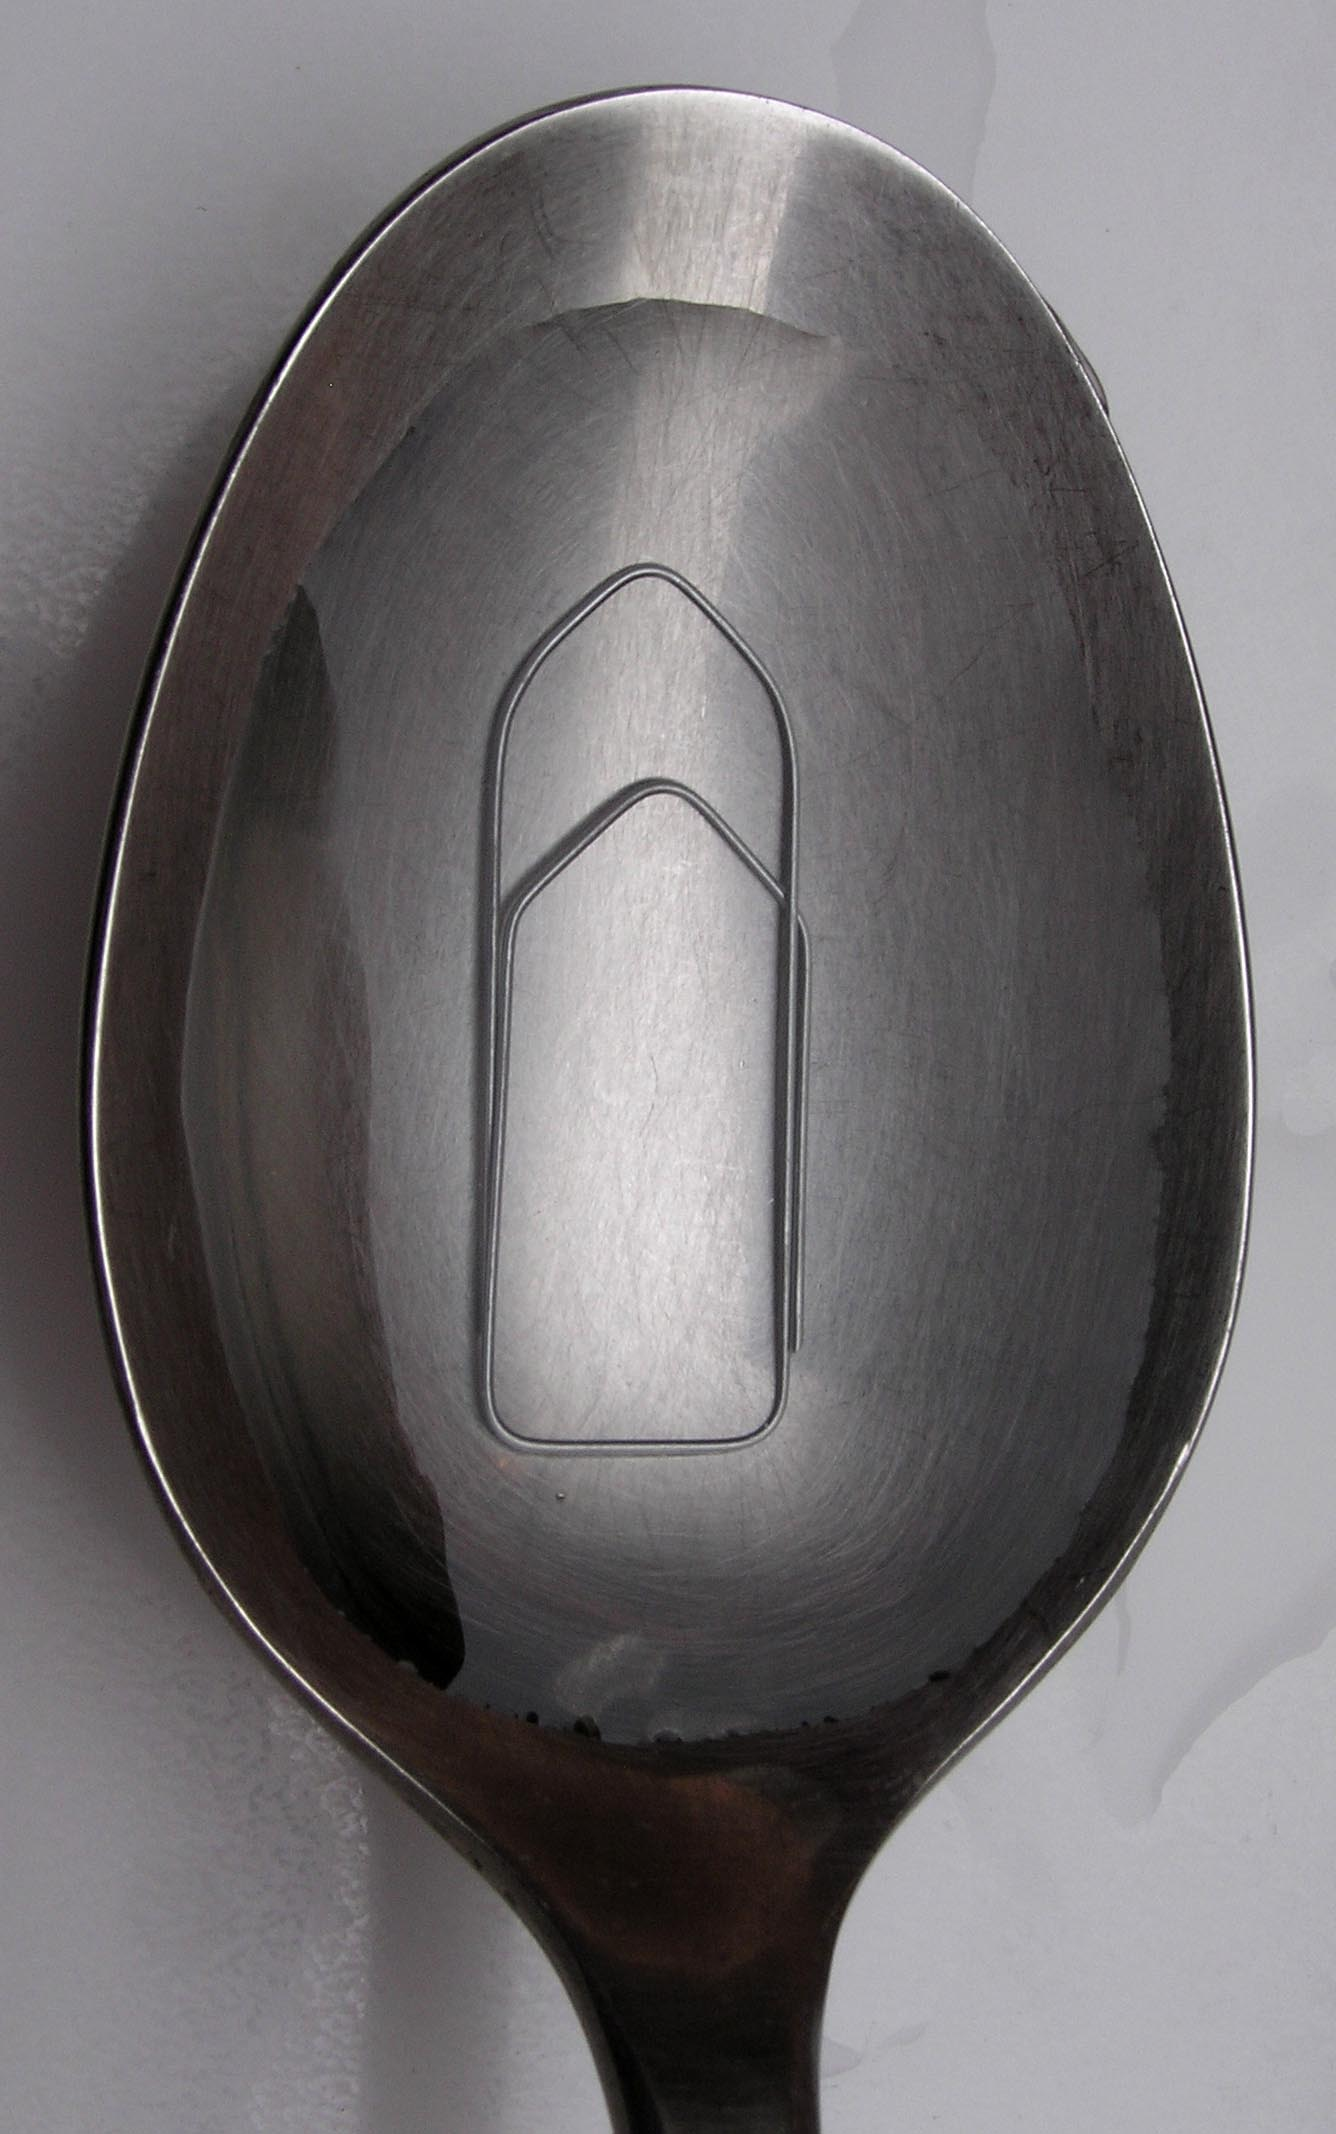
\includegraphics[width=0.5\textwidth]{medien/Nitinol_bueroklammer_heiss.jpg}
		\end{minipage}
	\end{figure}
 \end{frame}

\subsection{Effekte}
\label{fgl:effekte}
\begin{frame}[c]\frametitle{Effekte}
	Verschiedene Effekte von Formgedächtnislegierungen:
	\begin{itemize}
		\item{Einwegeffekt}
		\item{Zweiwegeffekt}
		\item{Pseudoelastizität}
	\end{itemize}
\end{frame}

\subsection{Vergleich}
\begin{frame}[c]\frametitle{Vergleich}
	\centering
	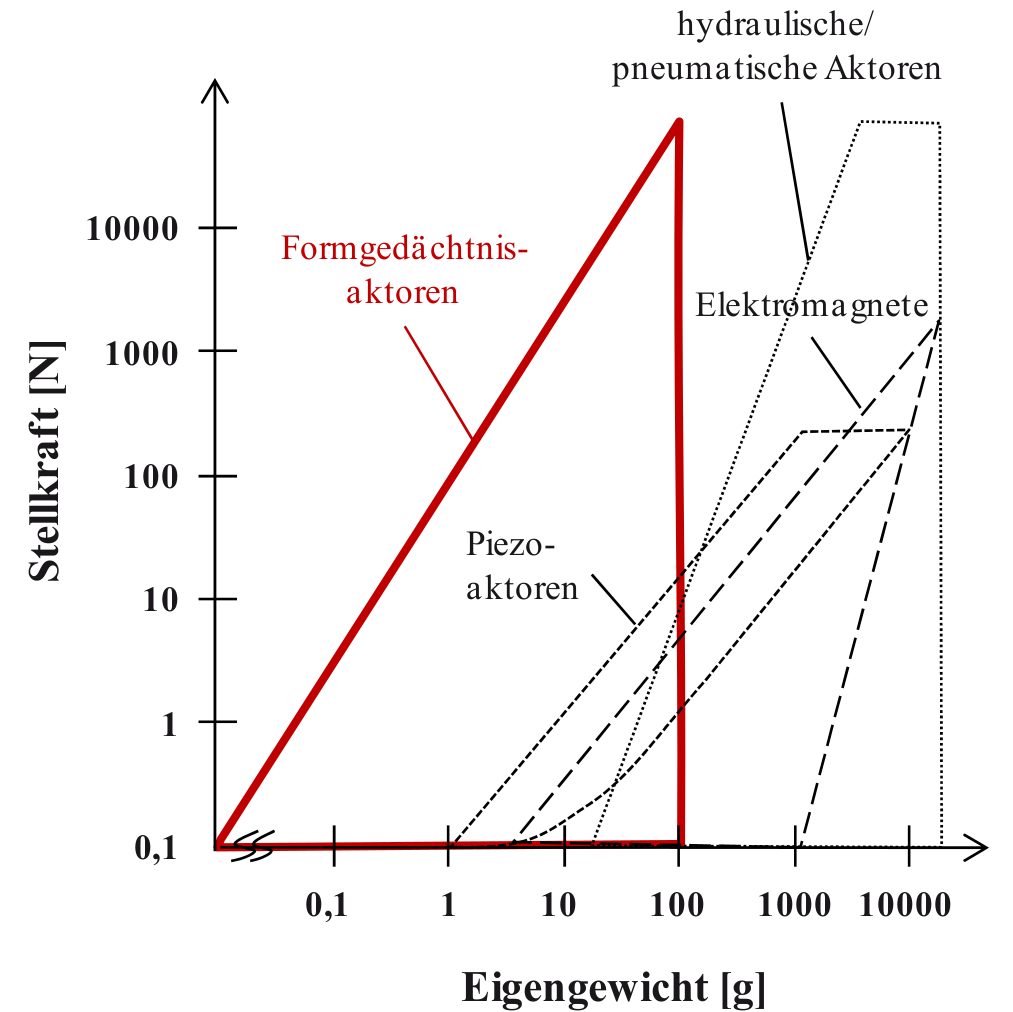
\includegraphics[height=0.5\textwidth]{medien/Verschiedene_Aktorprinzipien.png}
	\\
	\tiny{Quelle: Sven Langbein \& Alexander Czechowicz. Konstruktionspraxis
	Formgedächtnistechnik. Potentiale - Auslegung - Beispiele (Seite: 32).}
\end{frame}

\begin{frame}[c]\frametitle{Temperaturstrahl}
	\centering
	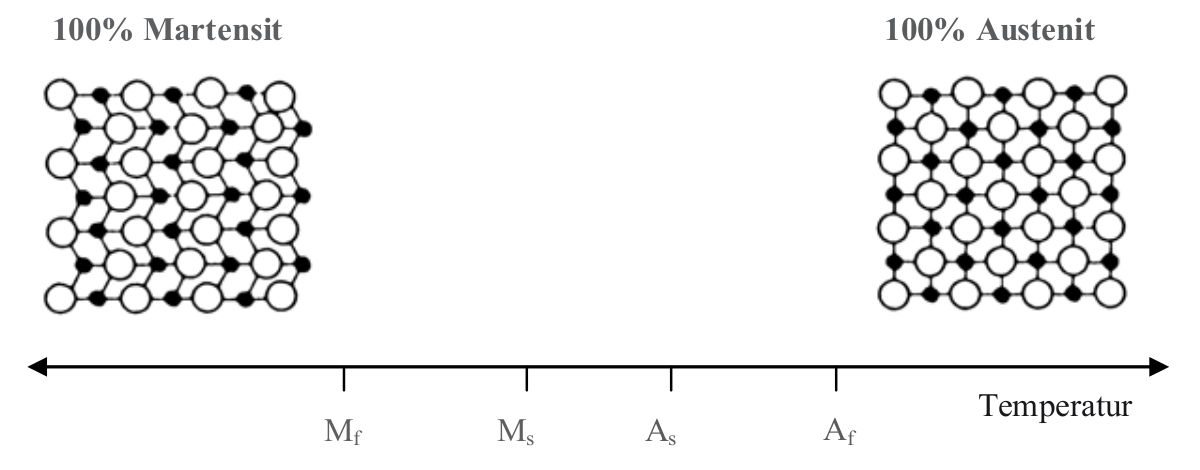
\includegraphics[height=0.35\textwidth]{medien/Umwandlung_anhand_des_Temperaturstrahls.png}
	\\
	\tiny{Quelle: Sven Langbein \& Alexander Czechowicz. Konstruktionspraxis
	Formgedächtnistechnik. Potentiale - Auslegung - Beispiele (Seite: 3).}
\end{frame}

\subsection{Einwegeffekt}
\begin{frame}[t]\frametitle{Einwegeffekt}
	\centering
	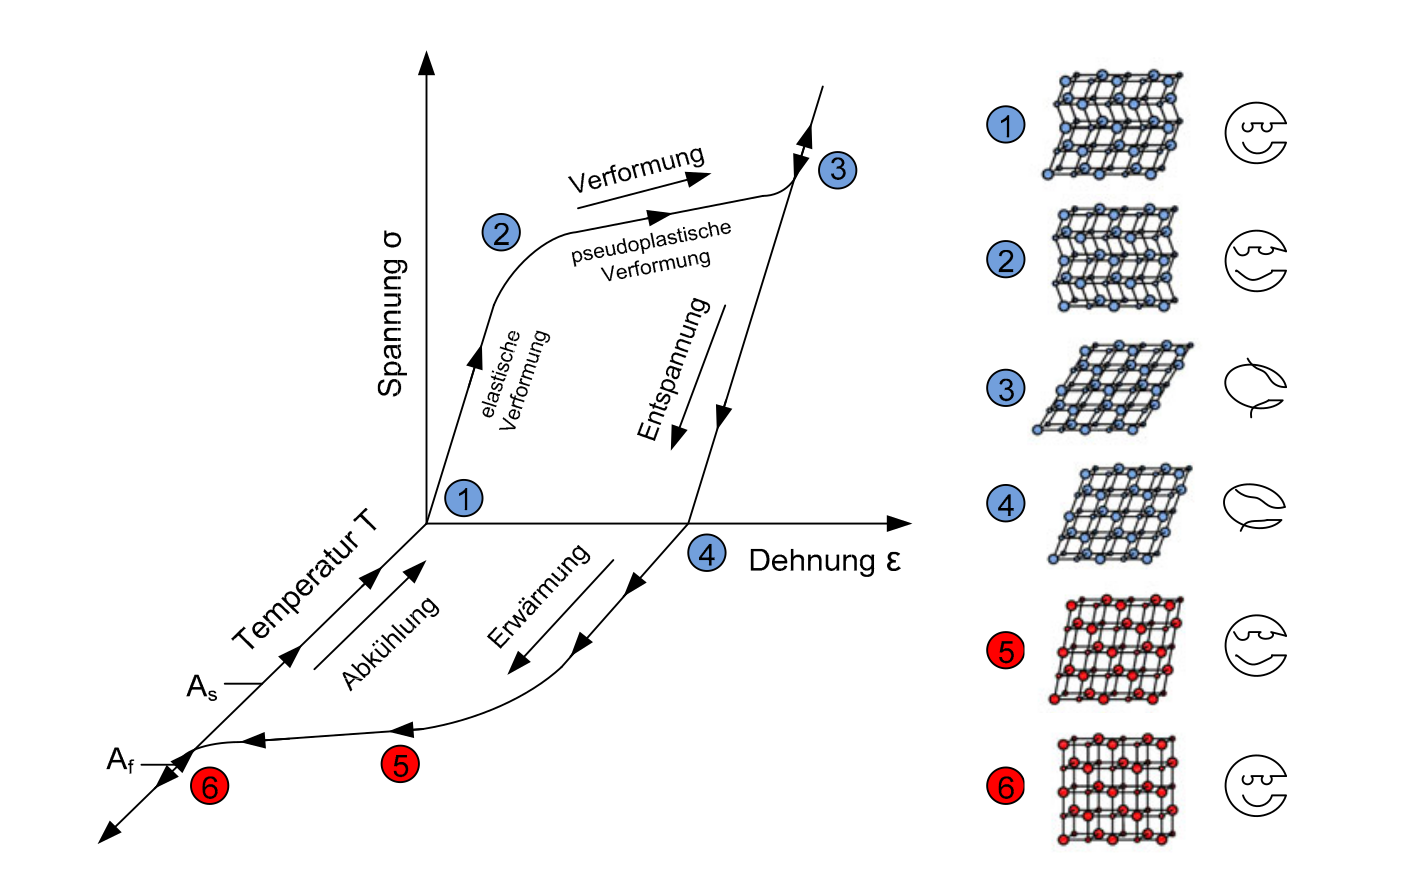
\includegraphics[height=0.5\textwidth]{medien/Verhalten_beim_Einwegeffekt.png}
	\\
	\tiny{Quelle: Sven Langbein \& Alexander Czechowicz. Konstruktionspraxis
	Formgedächtnistechnik. Potentiale - Auslegung - Beispiele (Seite: 6).}
\end{frame}

\subsection{Zweiwegeffekt}
\begin{frame}[t]\frametitle{Zweiwegeffekt}
	\centering
	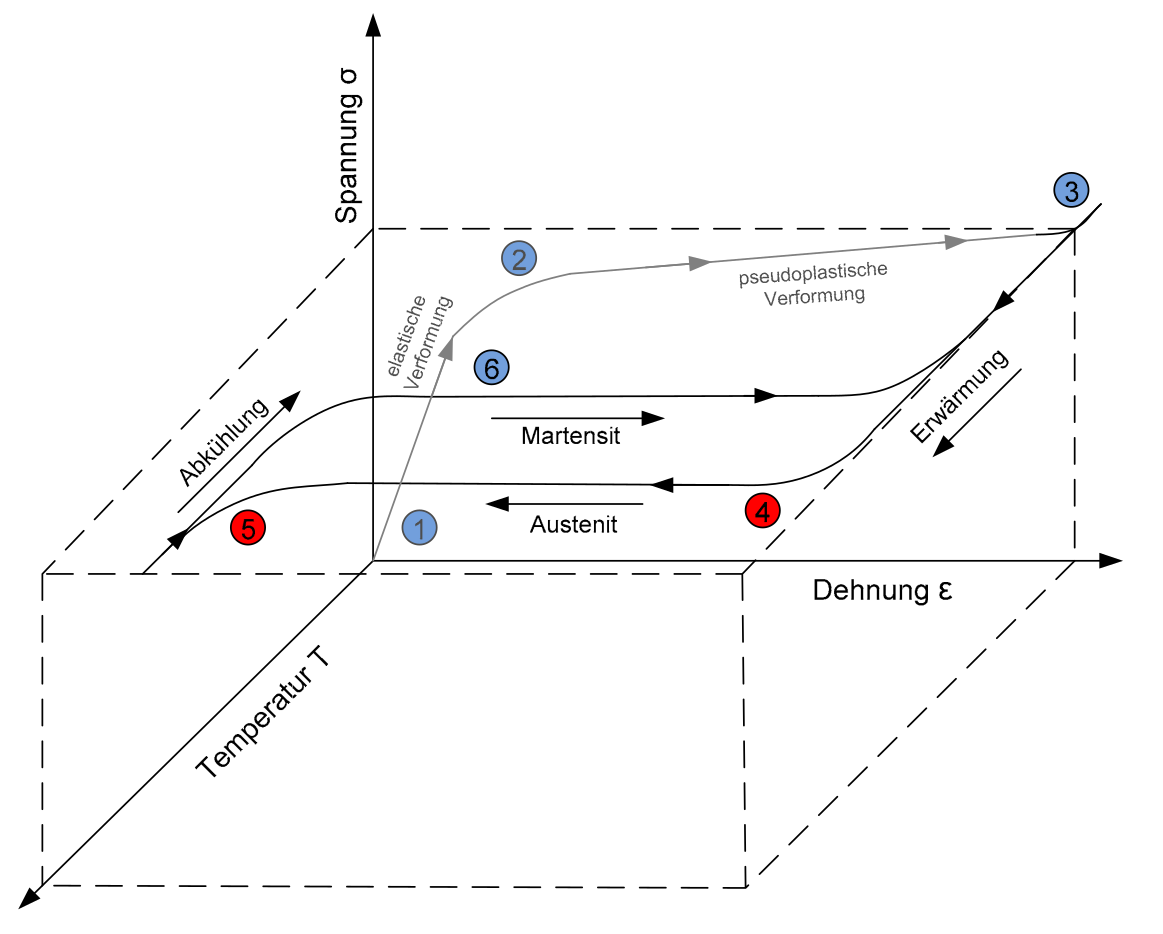
\includegraphics[height=0.5\textwidth]{medien/Verhalten_beim_Zweiwegeffekt.png}
	\\
	\tiny{Quelle: Sven Langbein \& Alexander Czechowicz. Konstruktionspraxis
	Formgedächtnistechnik. Potentiale - Auslegung - Beispiele (Seite: 7).}
\end{frame}

\subsection{Pseudoelastizität}
\begin{frame}[c]\frametitle{Pseudoelastizität}
	Die Umwandlungstemperatur liegt unter der Arbeitstemperatur
	(Umgebugstemperatur), im Normalfall unter 0°C.\\
	\centering
	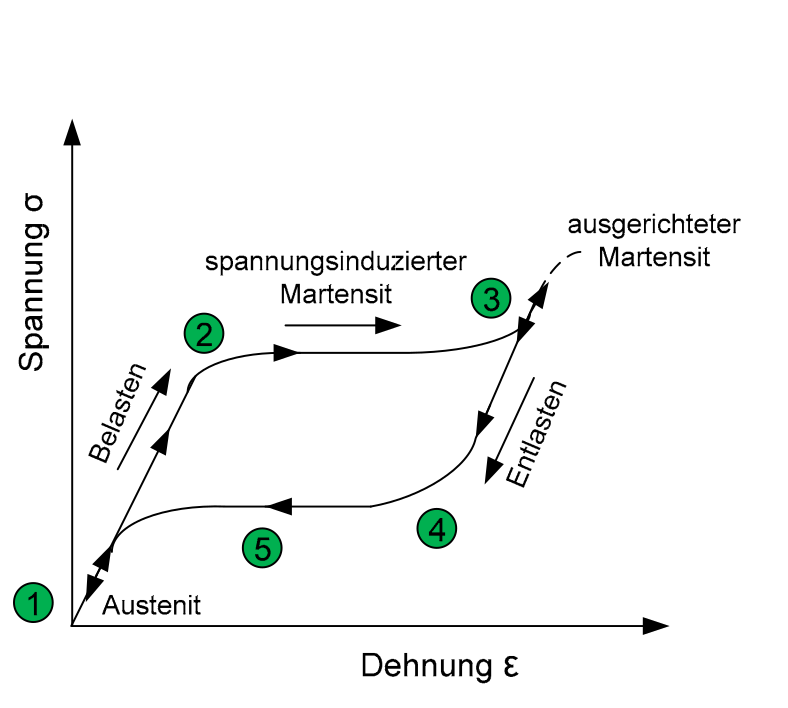
\includegraphics[height=0.5\textwidth]{medien/Verhalten_beim_pseudoelastischen_Effekt.png}
	\\
	\tiny{Quelle: Sven Langbein \& Alexander Czechowicz. Konstruktionspraxis
	Formgedächtnistechnik. Potentiale - Auslegung - Beispiele (Seite: 8).}
\end{frame}

\begin{frame}[c]\frametitle{Widerstandsänderung}
	\centering
	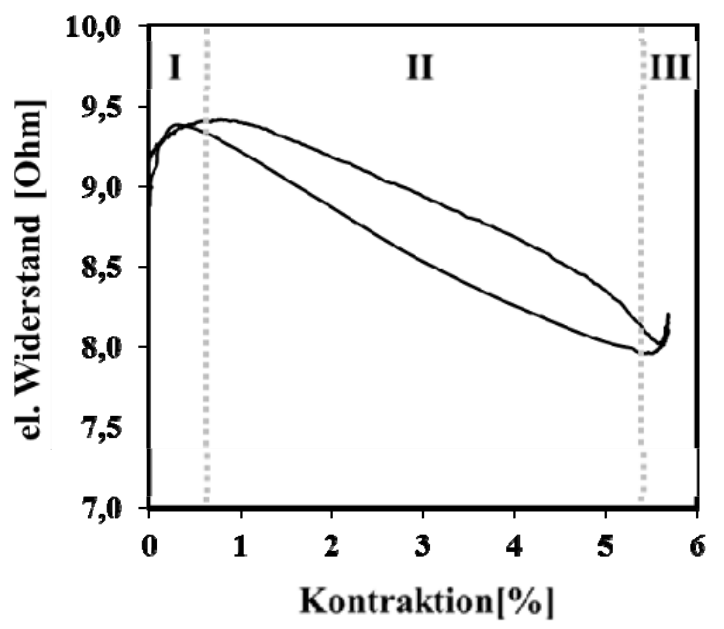
\includegraphics[height=0.5\textwidth]{medien/widerstand_zu_kontraktion.png}
	\\
	\tiny{Quelle: Sven Langbein \& Alexander Czechowicz. Konstruktionspraxis
	Formgedächtnistechnik. Potentiale - Auslegung - Beispiele (Seite: 110).}
\end{frame}

\subsection{Nutzbare FGL}
\begin{frame}[c]\frametitle{Nutzbare FGL}
	\centering
	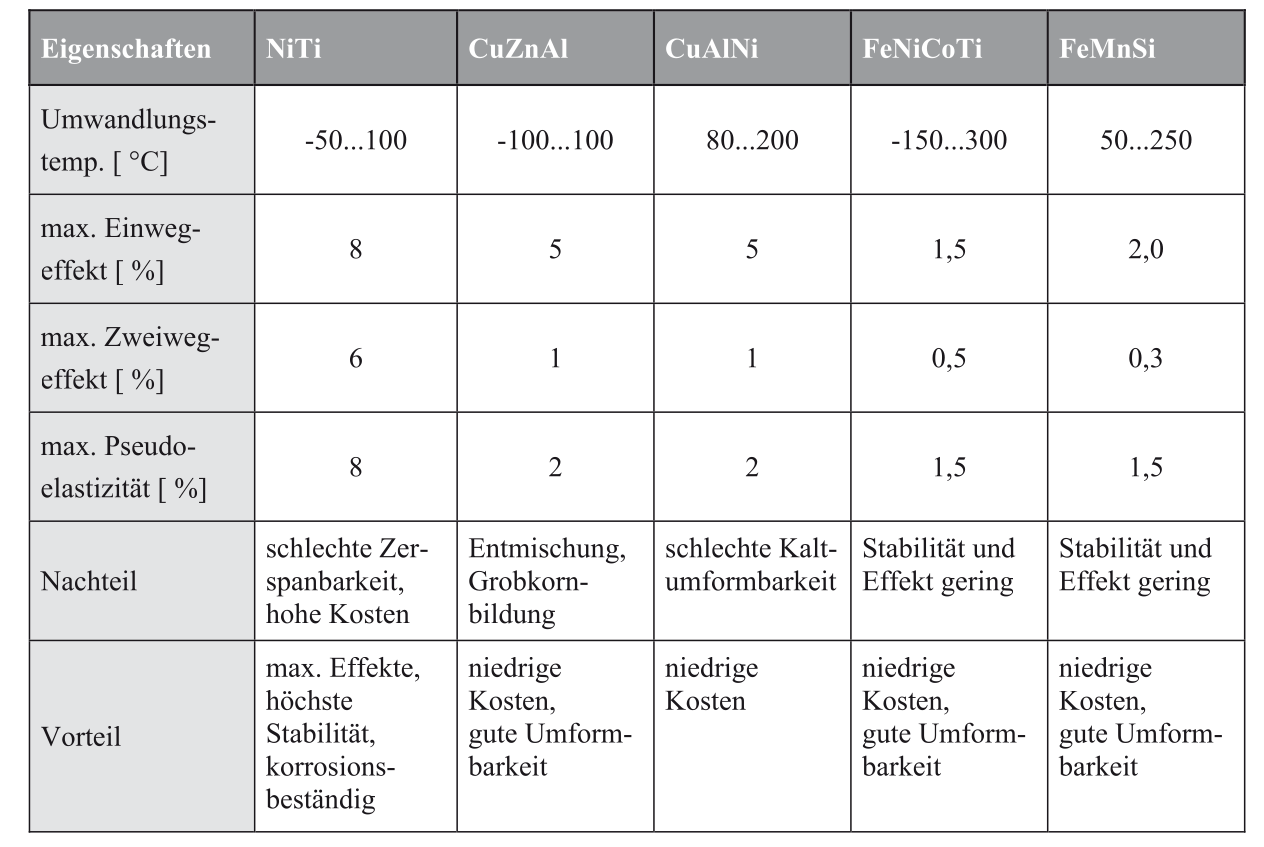
\includegraphics[height=0.5\textwidth]{medien/fgl_tabelle.png}
	\\
	\tiny{Quelle: Sven Langbein \& Alexander Czechowicz. Konstruktionspraxis
	Formgedächtnistechnik. Potentiale - Auslegung - Beispiele (Seite: 9).}
\end{frame}
